\documentclass[12pt,a4paper]{article}
\usepackage{listings}
\usepackage{lstlinebgrd}
\usepackage{graphicx}

\begin{document}

\title{Specification RFG V1.1}
\author{Tobias Markus}
\date{24.02.2015}

\maketitle

\tableofcontents
\newpage
\section{Introduction}
\section{RFG}
\subsection{RFG Language}
\subsection{RFG API}
\section{Generator API}
\subsection{User perspective}
\subsection{Developer perspective}
\section{RFG Verilog Generator}

\subsection{Overview}
\newpage
\subsection{Register}
Registers are the smallest addressable units in a registerFile. A register consists of one ore more fields with different widths and attributes. Depending on this variants hardware  will be generated. \\
\\
The different attributes and the resulting hardware is given in this subsection. 

\begin{lstlisting}[linewidth=\textwidth,language=tcl,basicstyle=\small,tabsize=4]
    ## A register with several fields and different attributes
    register test {
        field field_1 {
            width 32
            reset 32'h0
            software ro
            hardware wo
        }
        field field_2 {
            width 16
            reset 16'h0
            software rw
            hardware rw
        }
        field field_3 {
            width 16
            reset 16'h0
            software rw
        }

    }
\end{lstlisting}

The size of a register can be set with an attribute in the registerFile (register\_size). The default size of a register is 64 bit.

\newpage

\subsubsection{hardware/software Permissions}

The most common and important attributes are the permissions. A register has a software and a hardware interface. Each Interface can have read and/ or write permissions on a field in a register, defined with the attributes shown in the table below:\\
\\
\begin{tabular}{ l | r }
attribute name & description \\ \hline
ro & read only \\ \hline
wo & write only \\ \hline
rw & read and write \\ \hline
\end{tabular}
\\
\\
In this example we describe a register which has one 32 bit field with a reset value of zero and hardware read and write and software read and write permissions.\\
\\
RFG Description:
\lstinputlisting{specification_descriptions/reg_hrw_srw_hwen.rf}

Block Diagramm:
\begin{figure}[h!]
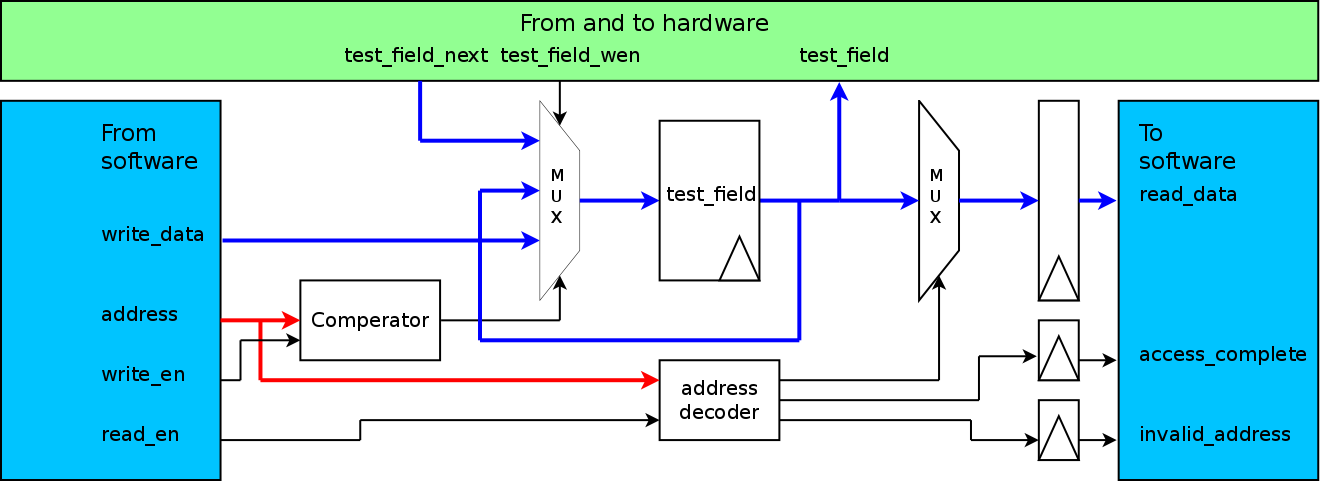
\includegraphics[width=0.92\textwidth]{pictures/Reg_hrw_srw_hwen.png}
\end{figure}
\newpage
Generated verilog from RFG description:
\lstinputlisting[linewidth=\textwidth,language=verilog,firstline=23,basicstyle=\small,tabsize=4,numbers=left,
linebackgroundcolor={
\ifnum\value{lstnumber}=16
    \color{yellow}
\fi
\ifnum\value{lstnumber}<40
    \ifnum\value{lstnumber}>29
        \color{yellow}
    \fi
\fi
\ifnum\value{lstnumber}=57
    \color{yellow}
\fi}
]
{specification_descriptions/verilog/reg_hrw_srw_hwen.v}
Depending on the permission attributes the verilog output is slightly different.\\
\\
The always block part from line 30 to line 39, represents the software write and hardware write functionality to one field. If the field has no software write permissions line 31 to line 34 are not generated. If the field has no hardware write permission line 35 to line 38 are not generated. If the field has neither a software write nor a hardware write only the reset logic is generated. If the field also does not have a reset attribute the always block is not generated. These descriptions without any hardware or software permissions are used to define reserved fields in a register.\\
\\
The hardware read is generated with the output reg on line 16 if there is no hardware read permission this signal is generated as internal reg.\\
\\
In the second always block the address decoder for the software read is generated. Depending on the read permission line 57 is generated or not.\\

\newpage

\subsubsection{no\_wen}

With the no\_wen attribute the hardware generator will not generate the hardware write enable signal on the register hardware interface. Attention when you write something with the software the hardware will rewrite the register in the next clock cycle.\\
\\
RFG Description:
\lstinputlisting{specification_descriptions/reg_hrw_srw_nhwen.rf}

Block Diagramm:
\begin{figure}[h!]
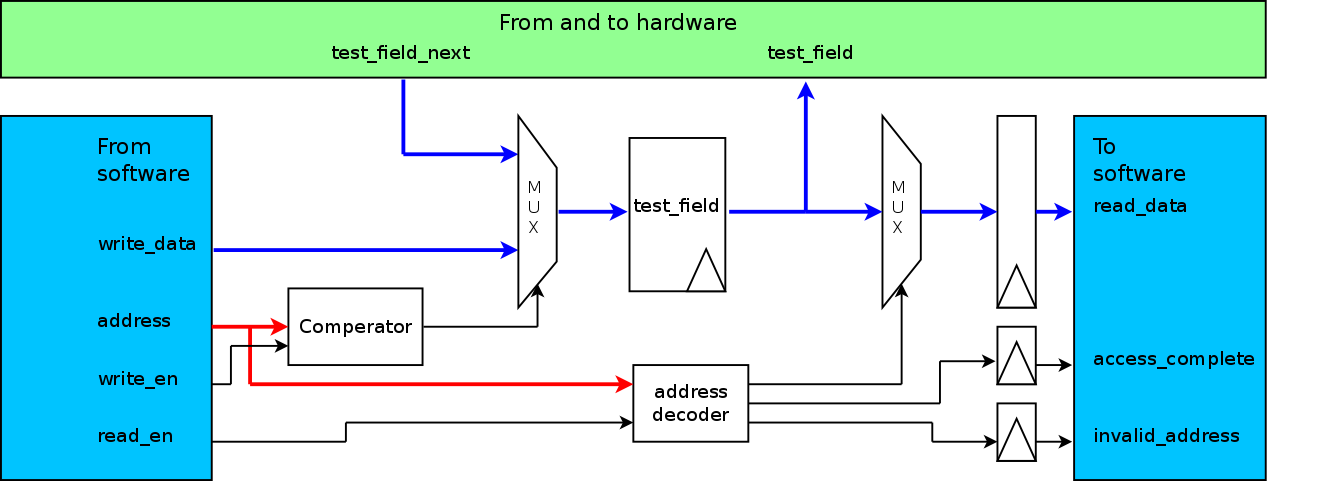
\includegraphics[width=0.92\textwidth]{pictures/Reg_hrw_srw_nhwen.png}
\end{figure}
\newpage
Generated verilog from RFG description:
\lstinputlisting[linewidth=\textwidth,language=verilog,firstline=23,basicstyle=\small,tabsize=4,numbers=left,
linebackgroundcolor={
\ifnum\value{lstnumber}=37
    \color{yellow}
\fi}
]{specification_descriptions/verilog/reg_hrw_srw_nhwen.v}
The difference in this verilog output can be observed in line 37. Now there is no hardware write enable signal. The register is written on each clock cycle. Keep this in mind if you write it via the software interface. The hardware has then one cycle to react to it and to rewrite the field.
\newpage

\subsubsection{write\_clear}
With the write\_clear attribute the field is cleared on a software write operation.\\
\\
RFG Descpription:
\lstinputlisting{specification_descriptions/reg_hrw_srw_swrite_clear.rf}

Block Diagramm:
\begin{figure}[h!]
    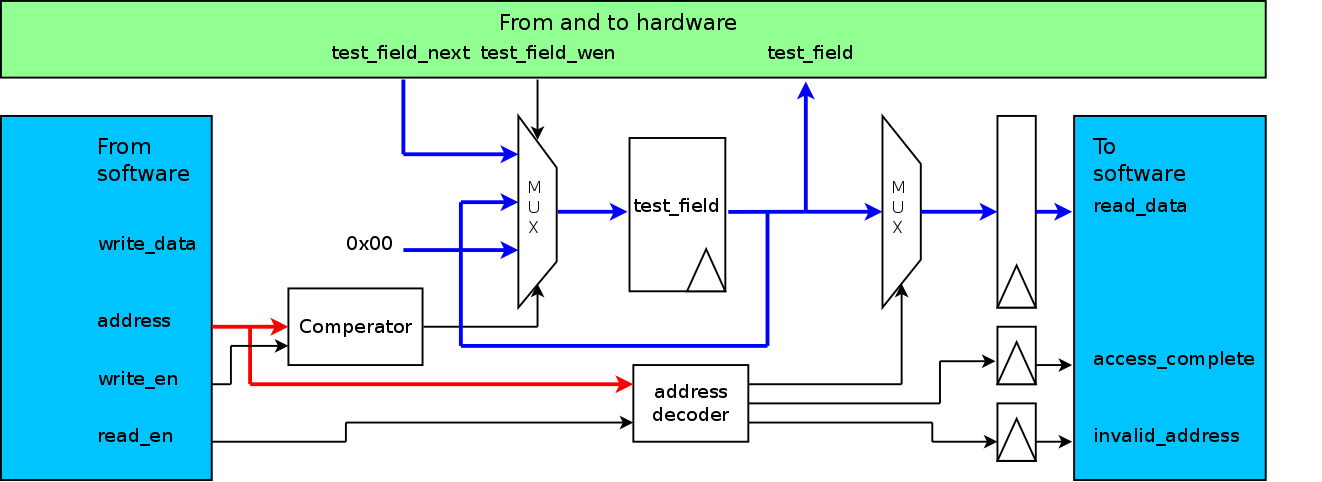
\includegraphics[width=\textwidth]{pictures/Reg_hrw_srw_swrite_clear.png}
\end{figure}
\newpage
Generated verilog from RFG description:
\lstinputlisting[linewidth=\textwidth,language=verilog,firstline=23,basicstyle=\small,tabsize=4,numbers=left,
linebackgroundcolor={
\ifnum\value{lstnumber}=33
    \color{yellow}
\fi}
]{specification_descriptions/verilog/reg_hrw_srw_swrite_clear.v}
In line 33 we can see that now the register is cleared when the register is written from the software.
\newpage

\subsubsection{software\_written}
With the software\_written signal an additional hardware output is generated which is high when the software writes the register. Otherwise the software\_written signal is low.\\
\\
RFG Description:
\lstinputlisting{specification_descriptions/reg_hrw_srw_swritten.rf}

Block Diagramm:
\begin{figure}[h!]
    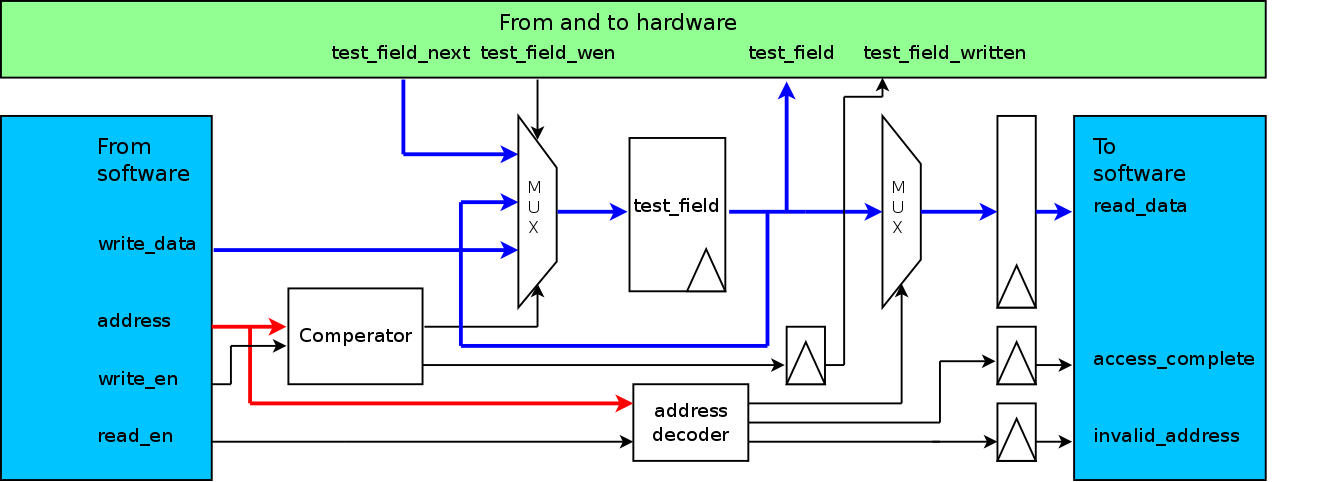
\includegraphics[width=\textwidth]{pictures/Reg_hrw_srw_swritten.png}
\end{figure}
\newpage
Generated verilog from RFG description:
\lstinputlisting[linewidth=\textwidth,language=verilog,firstline=23,basicstyle=\small,tabsize=4,numbers=left,
linebackgroundcolor={
\ifnum\value{lstnumber}=17
    \color{yellow}
\fi
\ifnum\value{lstnumber}=29
    \color{yellow}
\fi
\ifnum\value{lstnumber}=37
    \color{yellow}
\fi
\ifnum\value{lstnumber}=42
    \color{yellow}
\fi
\ifnum\value{lstnumber}<48
    \ifnum\value{lstnumber}>43
        \color{yellow}
    \fi
\fi}
]{specification_descriptions/verilog/reg_hrw_srw_swritten.v}
In this verilog output an additional hardware output signal is added (line 17). It is set when the software interface writes the field, line 34 to 38. It is reset on every cycle in which the software interface does not do a write operation.
\newpage
\subsubsection{changed}

The changed attribute behaves like the software\_written attribute described before. The only difference is that the changed signal is also set to high when the register is changed from a reset.\\
\\
RFG Description:
\lstinputlisting{specification_descriptions/reg_hrw_srw_changed.rf}

Block Diagramm:
\begin{figure}[h!]
    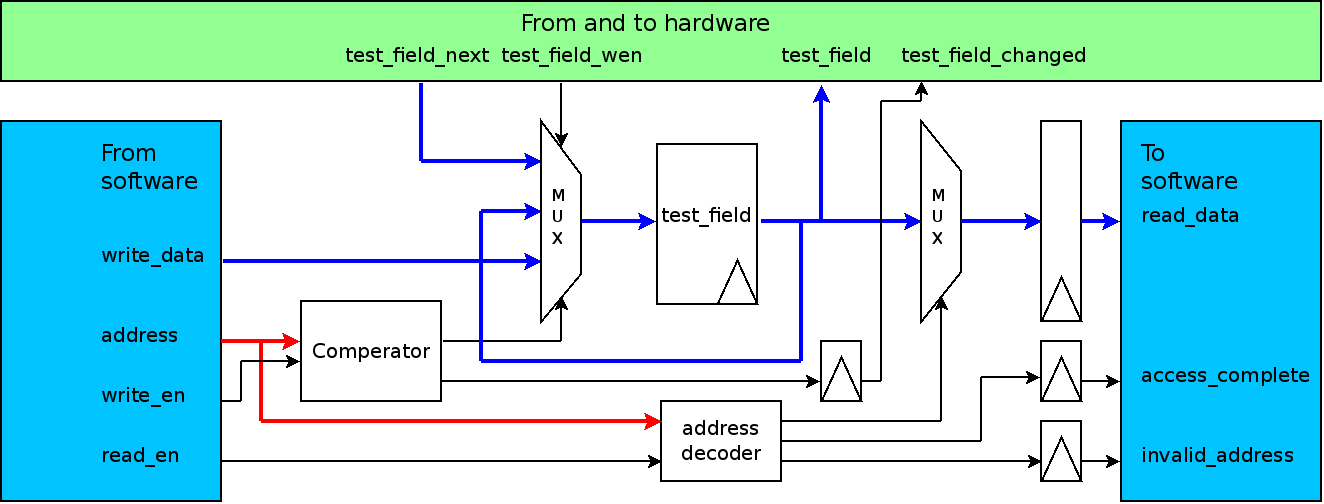
\includegraphics[width=\textwidth]{pictures/Reg_changed}
\end{figure}
\newpage

\subsubsection{sticky}
With the sticky feature a field is generated in which the bits in the field can only be set from the hardware. The field can only be reseted from the software interface or with a reset.\\
\\
RFG Description:
\lstinputlisting{specification_descriptions/reg_hrw_srw_sticky.rf}

Block Diagramm:
\begin{figure}[h!]
    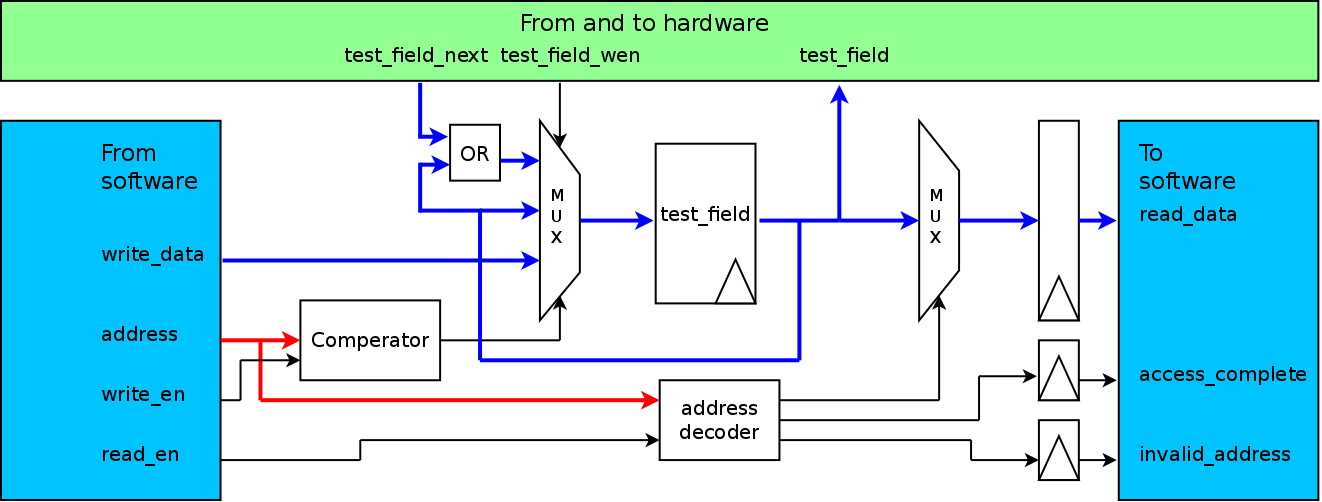
\includegraphics[width=\textwidth]{pictures/Reg_hrw_srw_sticky.png}
\end{figure}
\newpage
Generated verilog from RFG description:
\lstinputlisting[linewidth=\textwidth,language=verilog,firstline=23,basicstyle=\small,tabsize=4,numbers=left,breaklines=true,
linebackgroundcolor={
\ifnum\value{lstnumber}=38
    \color{yellow}
\fi}
]{specification_descriptions/verilog/reg_hrw_srw_sticky.v}
The difference in the verilog output with the sticky attribute is that the new hardware value is ored on write with the register value itself line 38.
\newpage

\subsubsection{software\_write\_xor}
The software\_write\_xor attributes writes on a software write the new value xored with the register value.\\
\\
RFG Description:
\lstinputlisting{specification_descriptions/reg_hrw_srw_swrite_xor.rf}

Block Diagramm:
\begin{figure}[h!]
    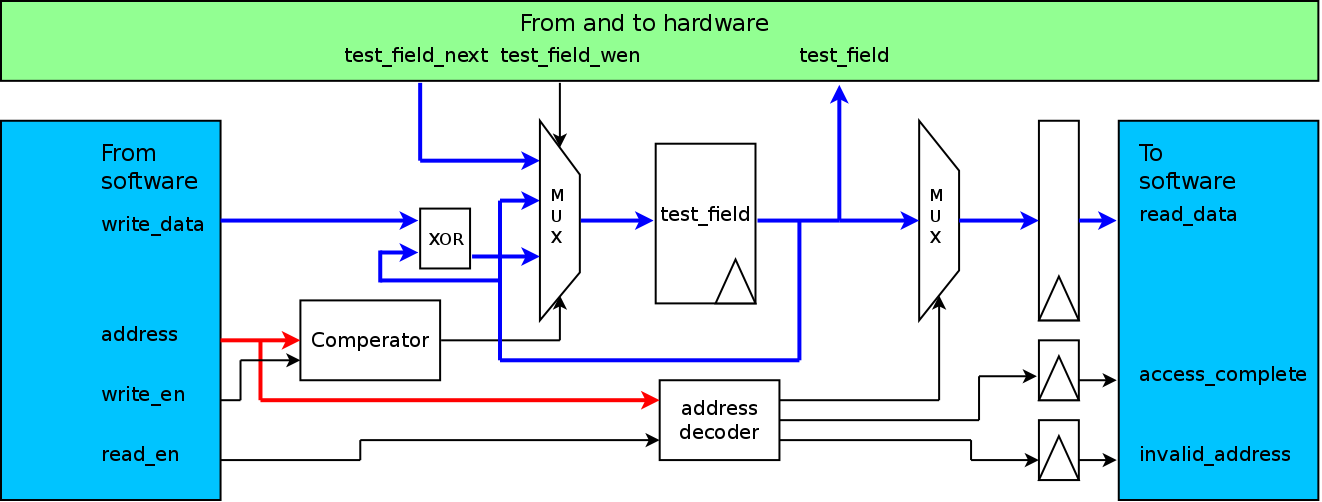
\includegraphics[width=\textwidth]{pictures/Reg_hrw_srw_swrite_xor.png}
\end{figure}
\newpage
Generated verilog from RFG description:
\lstinputlisting[linewidth=\textwidth,language=verilog,firstline=23,basicstyle=\small,tabsize=4,numbers=left,breaklines=true,
linebackgroundcolor={
\ifnum\value{lstnumber}=32
    \color{yellow}
\fi}
]{specification_descriptions/verilog/reg_hrw_srw_swrite_xor.v}
The software\_write\_xor attribute does also just do small change. When the register is written form the software interface it gets xored with itself line 32.
\newpage

\subsubsection{clear}
The hardware\_clear attribute adds an additional signal to the hardware interface. This signal clears the register when the hardware\_clear signal is asserted.\\
\\
RFG Description:
\lstinputlisting{specification_descriptions/reg_hrw_srw_hclear.rf}

Block Diagramm:
\begin{figure}[h!]
    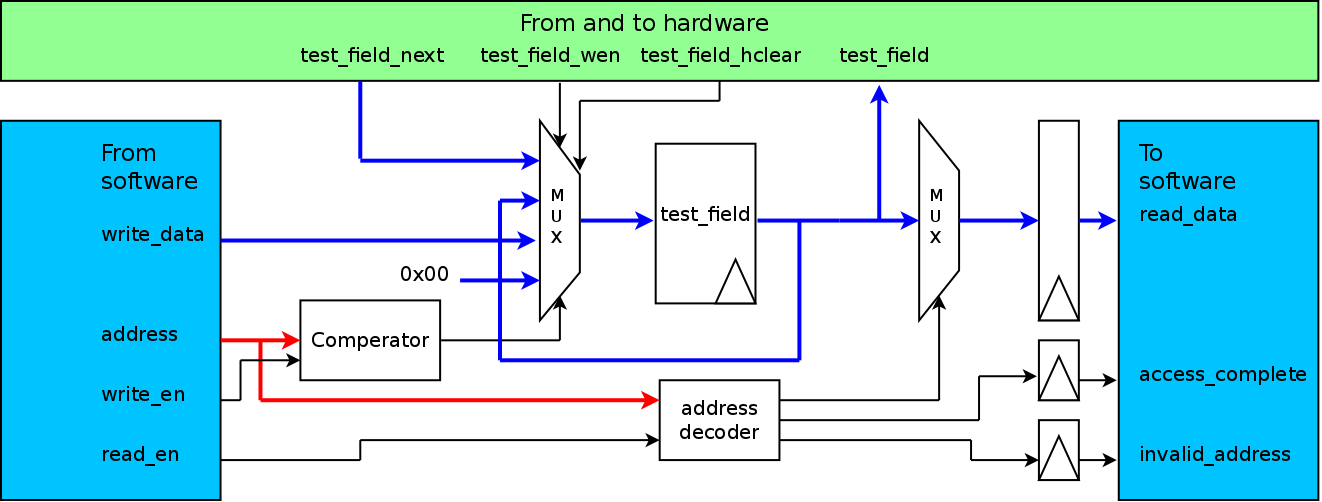
\includegraphics[width=\textwidth]{pictures/Reg_hrw_srw_hclear.png}
\end{figure}
\newpage
Generated verilog from RFG description:
\lstinputlisting[linewidth=\textwidth,language=verilog,firstline=23,basicstyle=\small,tabsize=4,numbers=left,breaklines=true,
linebackgroundcolor={
\ifnum\value{lstnumber}=17
    \color{yellow}
\fi
\ifnum\value{lstnumber}<38
    \ifnum\value{lstnumber}>33
        \color{yellow}
    \fi
\fi}
]{specification_descriptions/verilog/reg_hrw_srw_hclear.v}
\newpage

\subsubsection{trigger}

\subsubsection{counter}
The counter attribute transforms the internal register into a counter with count up signal for the hardware interface.\\
\\
RFG Description:
\lstinputlisting{specification_descriptions/reg_hrw_srw_counter.rf}

Block Diagramm:
\begin{figure}[h!]
    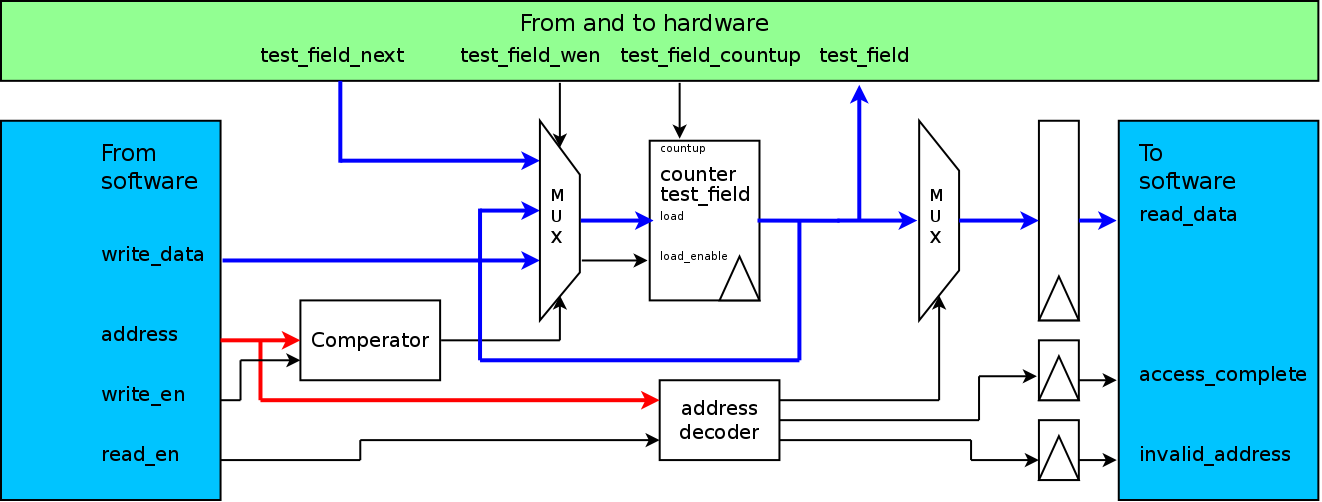
\includegraphics[width=\textwidth]{pictures/Reg_hrw_srw_counter.png}
\end{figure}
\newpage
Generated verilog from RFG description:
\lstinputlisting[linewidth=\textwidth,language=verilog,firstline=23,basicstyle=\small,tabsize=4,numbers=left,breaklines=true,
linebackgroundcolor={
\ifnum\value{lstnumber}=17
    \color{yellow}
\fi
\ifnum\value{lstnumber}<33
    \ifnum\value{lstnumber}>19
        \color{yellow}
    \fi
\fi
\ifnum\value{lstnumber}=39
    \color{yellow}
\fi
\ifnum\value{lstnumber}<48
    \ifnum\value{lstnumber}>45
        \color{yellow}
    \fi
\fi
\ifnum\value{lstnumber}<53
    \ifnum\value{lstnumber}>50
        \color{yellow}
    \fi
\fi
\ifnum\value{lstnumber}<58
    \ifnum\value{lstnumber}>55
        \color{yellow}
    \fi
\fi}
]{specification_descriptions/verilog/reg_hrw_srw_counter.v}
\newpage

\subsubsection{rreinit\_source, rreinit}
With the rreinit\_source and rreinit combination a register with the rreinit\_source attribute can be generated which resets a counter field marked with the rreinit attribute.\\
\\
RFG Description:
\lstinputlisting{specification_descriptions/reg_hrw_srw_rreinit_source.rf}
\newpage
Generated verilog from RFG description:
\lstinputlisting[linewidth=\textwidth,language=verilog,firstline=23,basicstyle=\small,tabsize=4,numbers=left,breaklines=true]{specification_descriptions/verilog/reg_hrw_srw_rreinit_source.v}
\newpage

\subsubsection{edge\_trigger}

\subsection{RamBlock}
A RamBlock is a construct which implements an addressspace as RAM inside the hardware. In different to registers, the hardware interface has now also address, data, and control lines. Depending on the read/write Permissions different RAMs are used. See the table below. 1w\_1r\_1c means a Ram with one write, one read interface. and 2rw\_1c means a dual port Ram.\\
\\
\begin{tabular}{ l || c | c | c | c | r }
    permissions & none & ro & wo & rw & hardware\\ \hline\hline
    none & none & none & none & 1w\_1r\_1c \\ \cline{1-5}
    ro & none & none & 1w\_1r\_1c& 2rw\_1c\\ \cline{1-5}
    wo & none & 1w\_1r\_1c& none & 2rw\_1c\\ \cline{1-5}
    rw & 1w\_1r\_1c& 2rw\_1c& 2rw\_1c & 2rw\_1c\\ \cline{1-5}
    software \\
\end{tabular}
\\
\\
RFG Description:
\lstinputlisting{specification_descriptions/RamBlock.rf} 
\newpage
Generated verilog from RFG description:
\lstinputlisting[linewidth=\textwidth,language=verilog,firstline=23,basicstyle=\small,tabsize=4,numbers=left,breaklines=true]{specification_descriptions/verilog/RamBlock.v}
\newpage
\subsubsection{attributes RamBlock}
external attribute:\\
\\
With the external attribute there is just a RamBlock Interface generated to communicate with a RamBlock outside the registerfile.\\
\\
address\_shift attribute:\\
\\
The address\_shift attributes allows to address the Ram Block with a shift inside the registerfile address space. In example each ramblock entry each 4kB with (address\_shift 12)
\newpage
\subsection{external/internal RegisterFiles}
A registerfile can be included in another one. There are two different constructs to include the registerfile internal or external.\\
\\
RFG Description:
\lstinputlisting{specification_descriptions/RF.rf}
\newpage
Generated verilog from RFG description:
\lstinputlisting[linewidth=\textwidth,language=verilog,firstline=23,basicstyle=\small,tabsize=4,numbers=left,breaklines=true]{specification_descriptions/verilog/RF.v}
\newpage

\end{document}
